\documentclass{article}
\usepackage[utf8]{inputenc}
\usepackage[T1]{fontenc}
\usepackage[spanish]{babel}
\usepackage{geometry}
\usepackage{graphicx}
\usepackage{float}
\usepackage{booktabs}
\usepackage{xltabular}   % longtable + tabularx
\geometry{a4paper, margin=1in}

\begin{document}

\begin{titlepage}
\IfFileExists{fig/logo-tec.png}{%
\begin{figure}[H]
    \centering
    \vspace{1cm}
    
\includegraphics[scale=0.6]{fig/logo-tec.png}
\end{figure}
}{}
    \centering
    \vspace*{-0.5cm}

    {\Large\bfseries Escuela de Ingeniería Electrónica\par}
    \vspace{1em}

    {\Large\bfseries Verificación Funcional de Circuitos Integrados\par}
    \vspace{4cm}

    {\Large\bfseries Proyecto I:\@ Test Plan.\par}

    \vspace{4cm}

    \large
    Luis Diego Garcia Rojas \textendash{} 2020124283\\
    Cristhian Lezcano Fernández \textendash{} 2018111011\\
    \vfill
    II Semestre 2026

\end{titlepage}


% =====================================================================
\section*{Descripción del dispositivo}
% =====================================================================

El dispositivo bajo prueba es un bus de comunicación serial compartido al
que se conectan cuatro dispositivos y cuya función es enrutar paquetes de
datos entre ellos. Como la línea de datos es común a todos, solo uno puede
transmitir a la vez y el turno se reparte de forma rotativa.

Este arbitraje no es centralizado, sino que cada dispositivo lleva su
propio registro del turno actual y todos se mantienen sincronizados
mediante una línea de control que indica el cambio de turno, de modo que
el acceso se reparte de forma equitativa sin que exista un árbitro único.
Los identificadores válidos son 0 a 3, el identificador de difusión es 255
y las direcciones 4 a 254 no corresponden a ningún dispositivo. Las FIFOs
de entrada y salida son emuladas por el ambiente de verificación y no
forman parte del dispositivo bajo prueba.




\subsection*{Ambiente de verificación}

El ambiente instancia un driver por cada dispositivo del bus. El Test
genera los paquetes y los entrega al Agente, que los reparte entre los
drivers; cada driver escribe en la FIFO de salida de su dispositivo y
recibe lo que el bus deposita en la FIFO de entrada. El Checker recoge lo
observado por los drivers y el Scoreboard lo contrasta contra los
paquetes que el Test generó. Las aserciones vigilan el protocolo de la
línea serial y el cambio de turno.

\begin{figure}[H]
    \centering
    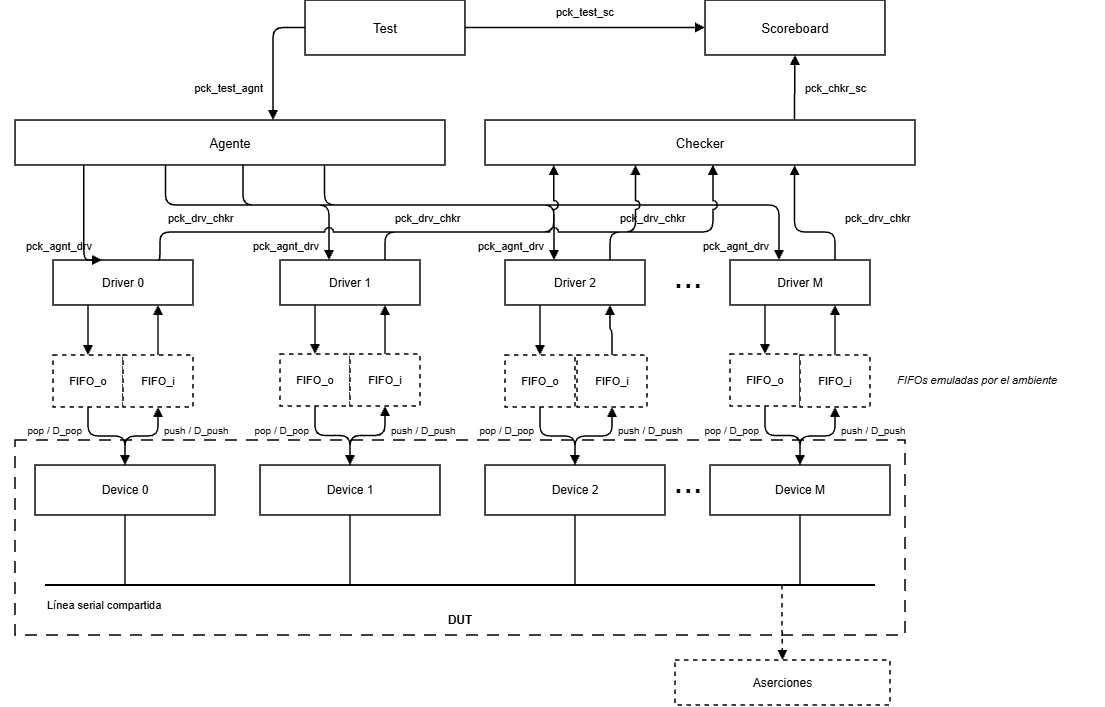
\includegraphics[width=\textwidth]{fig/ambiente.png}
    \caption{Bloques del ambiente de verificación y paquetes de
    comunicación entre ellos.}
    \label{fig:ambiente}
\end{figure}


% =====================================================================
\section*{Test Plan}
% =====================================================================

Los casos identificados con el prefijo \texttt{TG} corresponden a Casos
Generales y los identificados con \texttt{TE} a Casos de Esquina.

\renewcommand{\arraystretch}{1.15}
\footnotesize

\begin{xltabular}{\textwidth}{%
  >{\bfseries\raggedright\arraybackslash}p{0.11\textwidth}
  >{\raggedright\arraybackslash}X
  >{\raggedright\arraybackslash}X
  >{\raggedright\arraybackslash}X
  >{\raggedright\arraybackslash}X}

\toprule
\textbf{Nombre} & \textbf{Qué se prueba} & \textbf{Qué se hace} &
\textbf{Aleatorización y rangos} & \textbf{Criterio de aprobación} \\
\midrule
\endfirsthead

\toprule
\textbf{Nombre} & \textbf{Qué se prueba} & \textbf{Qué se hace} &
\textbf{Aleatorización y rangos} & \textbf{Criterio de aprobación} \\
\midrule
\endhead

\bottomrule
\endlastfoot

\multicolumn{5}{l}{\normalsize\itshape Casos generales} \\
\cmidrule(r){1-5}

TG-01 Transmisión simple y secuencial
& Enrutamiento del paquete al destino indicado e integridad del
  contenido.
& Un transmisor activo por vez; el \emph{scoreboard} compara lo emitido
  contra lo recibido en cada interfaz.
& Datos transmitidos: uniforme sobre todo el ancho.\newline
  Origen y destino: 0--3, con origen distinto del destino.\newline
  Tiempos de envío: 0--20 ciclos.\newline
  Paquetes por dispositivo: 100.
& El contenido recibido coincide exactamente con el enviado, llega
  únicamente al destino indicado y se conserva el orden correcto de los
  paquetes en el \emph{scoreboard}. \\
\midrule[0.02em]

TG-02 Anchos de paquete
& Soporte de los tres anchos y decodificación de la dirección en los
  8 bits más significativos.
& Transacciones con anchos mezclados dentro de la misma prueba, forzando
  cambios entre paquetes consecutivos.
& Largo de los paquetes: $\{16, 32, 64\}$ bits, uniforme.\newline
  Datos transmitidos: uniforme sobre los bits restantes.\newline
  Cambios de ancho: $\geq 20$ por prueba.
& El contenido se preserva íntegro en los tres anchos y la dirección se
  interpreta correctamente en los 8 bits más significativos. \\
\midrule[0.02em]

TG-03 Reset del sistema
& Retorno a un estado conocido desde cualquier punto de la operación,
  incluido el reset a mitad de una transmisión.
& Activación del reset en tres escenarios: bus en reposo, paquete en
  vuelo y cambio de turno.
& Momento de activación: uniforme dentro de una transacción
  completa.\newline
  Duración del pulso: 1--5 ciclos.\newline
  Escenario: uniforme entre los tres.
& Todas las interfaces arrancan en un estado conocido, el bus queda
  disponible y no se reportan paquetes espurios. \\
\midrule[0.02em]

TG-04 Rotación del turno
& Equidad del arbitraje distribuido: ningún dispositivo monopoliza el bus
  ni queda sin acceso.
& Tráfico sostenido desde los cuatro dispositivos; se cuentan las
  concesiones obtenidas por cada uno.
& Ocupación por dispositivo: 0\,\%--100\,\%.\newline
  Rondas observadas: $\geq 50$.\newline
  Instante de arranque: 0--10 ciclos.
& La diferencia entre dispositivos no supera una concesión por ronda y
  ninguno accede al bus fuera de su turno. \\
\midrule

\multicolumn{5}{l}{\normalsize\itshape Casos de esquina} \\
\cmidrule(r){1-5}

TE-01 Transmisión broadcast
& Replicación del paquete a todos los dispositivos cuando el destino es
  el identificador de difusión.
& Paquetes dirigidos al identificador 255, intercalados con tráfico
  dirigido a un solo destino.
& Identificador de broadcast: 5\,\%--30\,\% de los paquetes.\newline
  Origen: 0--3.\newline
  Largo y datos: como en TG-02.
& Todos los dispositivos reciben una copia exacta del paquete y el turno
  avanza con normalidad. \\
\midrule[0.02em]

TE-02 Acceso simultáneo
& Resolución de la contención cuando todos los dispositivos solicitan el
  bus en el mismo ciclo.
& Retardos de inicio alineados para que las solicitudes de acceso
  coincidan exactamente.
& Dispositivos en contención: 2--4.\newline
  Eventos por prueba: 10--50.\newline
  Tiempo de acceso al bus: forzado al mismo ciclo.
& El arbitraje resuelve la contención sin perder paquetes y todos los
  transmisores obtienen el bus respetando su turno correspondiente. \\
\midrule[0.02em]

TE-03 Mensajes con direcciones inválidas
& Que un destino inexistente no bloquee el bus ni detenga la rotación.
& Envío de paquetes hacia direcciones no configuradas, intercalados con
  tráfico válido.
& Mensajes con error de direccionamiento: 5\,\%--20\,\%.\newline
  Dirección destino: uniforme en 4--254.
& Ningún dispositivo acepta el paquete; el mensaje consume su tiempo de
  bus, pero luego el bus queda liberado y las transacciones posteriores
  se completan con normalidad. \\
\midrule[0.02em]

TE-04 Overflow de la FIFO
& Detección de la condición de FIFO de entrada llena, emulada por el
  ambiente de verificación.
& Tráfico continuo desde varios transmisores hacia un mismo destino hasta
  llenar por completo su FIFO de entrada.
& Dirección de destino: sesgada, 70\,\%--90\,\% hacia un mismo
  receptor.\newline
  Receptor saturado: 0--3.\newline
  Tiempos de envío: 0--2 ciclos.
& El ambiente detecta la condición de FIFO llena y actúa según el
  comportamiento definido, sin que se generen paquetes corruptos en el
  \emph{scoreboard}. \\
\midrule[0.02em]

TE-05 Underflow de la FIFO
& Cesión del turno cuando corresponde transmitir y la FIFO de salida está
  vacía.
& Generación de ventanas prolongadas sin paquetes pendientes para que el
  turno llegue con la FIFO vacía.
& Tiempos de envío: 20--200 ciclos.\newline
  Número de transacciones: 0--10 por dispositivo.\newline
  Dispositivos inactivos: 1--3.
& El dispositivo sin paquetes cede su turno sin transmitir datos erróneos
  y la rotación del bus continúa con normalidad entre los demás
  dispositivos conectados. \\
\midrule[0.02em]

TE-06 Sincronía del turno
& Que los registros locales de turno de los cuatro dispositivos coincidan
  en todo momento.
& Monitor pasivo que muestrea el registro de turno de cada interfaz en
  cada flanco y los compara entre sí.
& Momento del reset: uniforme dentro de una ronda.\newline
  Incorporación de cada dispositivo: 0--3 rondas.
& Los registros coinciden en todos los ciclos posteriores a la
  sincronización y nunca hay dos dispositivos con el mismo turno. \\

\end{xltabular}

\end{document}